En esta sección, revisamos
brevemente~\citep{choksi_partial_2022,salgado_classical_2022} los
conceptos asociados a un problema de valor de frontera y su solución.
Luego, derivaremos la ecuación de advección-difusión unidimensional
según~\citep{leveque_numerical_1992}.
Finalmente, mostramos el método de las líneas para convertir nuestra
ecuación de interés en un sistema de ecuaciones diferenciales
ordinarias.

\section{GENERALIDADES}

\begin{definition}[Ecuación Diferencial Parcial (EDP)]
    Es una ecuación que involucra una \emph{función desconocida} $u$
    y sus derivadas parciales junto con las variables independientes.
    Se escribe como
    \begin{equation}
        \mathcal{L}
        \left(
        \text{variables independientes},
        u,
        \text{derivadas de $u$}
        \right)
        =0.
        \label{eq:pde}
    \end{equation}
\end{definition}

\begin{definition}[Dominio]
    Un dominio $\Omega$ es un subconjunto de $\mathbb{R}^{d}$ abierto
    y conexo que tiene frontera lineal a trozos de clase $C^{1}$.
\end{definition}

En lo sucesivo $\Omega$ siempre será un dominio.

\begin{definition}[Solución clásica de la EDP]
    Es una función $u\colon\Omega\to\mathbb{R}$ suficientemente suave
    que satisface~\eqref{eq:pde} para cualquier $x\in\Omega$.
\end{definition}

\begin{definition}[Condiciones auxiliares]
    Una \emph{condición auxiliar} en una solución general es una
    igualdad que especifica el valor de la función desconocida en un
    subconjunto de $\Omega$.
\end{definition}

\begin{definition}[Problema de Valor Inicial (PVI)]
    Sea
    \begin{math}
        u\colon
        \Omega\times\left[0,T\right]
        \to\mathbb{R}
    \end{math}
    una solución de~\eqref{eq:pde}.
    Un \emph{problema de valor inicial} es una ecuación diferencial
    junto con un conjunto de condiciones auxiliares que especifican
    la solución y/o sus derivadas en $t=0$.
\end{definition}

\begin{example}[PVI de la ecuación de difusión]
    \begin{equation*}
        \begin{cases}
            \difcp{u}{t}=
            \alpha^{2}
            \difc.L.{u}{}  &
            \text{ para }
            \left(x,t\right)\in
            \Omega\times\left[0,T\right]. \\
            u
            \left(x,0\right)=
            \phi
            \left(x\right),\quad
            \difcp{u}{t}
            \left(x,0\right)=
            \psi
            \left(x\right) &
            \text{ para }
            x\in\Omega.
        \end{cases}
    \end{equation*}
\end{example}

\begin{definition}[Problema de Valor de Frontera (PVF)]
    Sea
    \begin{math}
        u\colon
        \Omega
        \to\mathbb{R}
    \end{math}
    una solución de~\eqref{eq:pde}.
    Un \emph{problema de valor de frontera} es una ecuación
    diferencial junto con un conjunto de condiciones auxiliares que
    especifican la solución y/o sus derivadas en $\partial\Omega$.
\end{definition}

\begin{example}[Problema de valor de frontera de la ecuación de Laplace]
    \begin{equation*}
        \begin{cases}
            \difc.L.{u}{}=0
             & \text{ para }
            \left(x,y\right)\in\Omega. \\
            u=f
             & \text{ en }
            \partial\Omega.
        \end{cases}
    \end{equation*}
\end{example}

\begin{definition}[Problema bien planteado]
    Es una EDP con condiciones auxiliares que cumple
    \begin{description}
        \item[Existencia.]

            Para una elección de la condición auxiliar, existe
            una solución para la EDP que lo satisface.

        \item[Unicidad.]

            Solo existe una solución.

        \item[Estabilidad.]

            Si perturbamos poco una condición auxiliar, la nueva
            solución no cambia mucho respecto a la solución original.
    \end{description}
\end{definition}

\begin{definition}[Clasificación de la EDP lineal de segundo orden]
    Sea la EDP lineal de segundo orden con coeficientes constantes
    \begin{math}
        \mathcal{L}u\left(x\right)=
        f\left(x\right)
    \end{math}
    y $x\in\Omega$, donde el operador diferencial $\mathcal{L}$ viene
    dado por
    \begin{align*}
        \mathcal{L}
        u\left(x\right) & \coloneqq
        \sum_{i,j=1}^{d}
        a_{ij}
        \difcp[2]{u}{ij}\left(x\right)+
        \sum_{i=1}^{d}
        b_{i}
        \difcp{u}{i}\left(x\right)+
        cu\left(x\right)            \\
                        & =
        {
        \inner{A}{\mathrm{D}^{2}u\left(x\right)}
        }_{F}+
        \inner{b}{\nabla u\left(x\right)}+
        c
        u\left(x\right),
    \end{align*}
    donde $A=\left[a_{ij}\right]\in\mathbb{R}^{d\times d}$,
    \begin{math}
        b={\left[b_{i}\right]}^{T}\in\mathbb{R}^{d}
    \end{math},
    \begin{math}
        \mathrm{D}^{2}u\left(x\right)
    \end{math}
    es la matriz hessiana de $u$ en $x$,
    \begin{math}
        \nabla u\left(x\right)
    \end{math}
    es el gradiente de $u$ en el mismo punto y el producto interno de
    Frobenius es definido como
    \begin{equation*}
        \forall A,B\in\mathbb{R}^{d\times d}:
        {\inner{A}{B}}_{F}\coloneqq
        \operatorname{tr}
        \left(A^{T}B\right).
    \end{equation*}
    Decimos que el operador diferencial parcial de segundo orden con
    coeficientes constantes $\mathcal{D}$ es
    \begin{description}
        \item[Elíptico:]

            Si los $d$ autovalores de $A$ tienen el mismo signo, es
            decir, o bien
            \begin{math}
                \sigma\left(A\right)\subset\mathbb{R}_{+}
            \end{math}
            o
            \begin{math}
                \sigma\left(A\right)\subset\mathbb{R}_{-}
            \end{math}.

        \item[Parabólico:]

            Si $A$ contiene exactamente $d-1$ valores propios o bien
            positivos o negativos y cero es un valor propio de
            multiplicidad uno.

        \item[Hiperbólico:]

            Si $A$ tiene $d-1$ valores propios positivos o negativos,
            y el restante es distinto de cero y de signo opuesto.

        \item[Ultra parabólico:]

            Si cero es un valor propio múltiple y todos los restantes
            tienen el mismo signo.

        \item[Ultra hiperbólico:]

            Si cero no es un valor propio y hay más de un valor
            propio positivo y más de un valor propio negativo.
    \end{description}
\end{definition}

\begin{example}[EDPs lineales de segundo orden]
    Sea $d\in\mathbb{N}$ la dimensión espacial.
    \begin{description}
        \item[Elíptica:]

            \begin{equation*}
                -\difc.L.{u}{}\left(x\right)=
                {
                \inner{
                -I_{d}
                }{
                \mathrm{D}^{2}u\left(x\right)
                }
                }_{F}=
                -\sum_{i=1}^{d}
                \difcp[2]{u}{i}\left(x\right)
            \end{equation*}

        \item[Parabólica:]

            \begin{equation*}
                H
                \left(x,t\right)=
                \difcp{u}{t}\left(x,t\right)+
                {\inner{
                    \begin{bmatrix}
                        -I_{d}         & \mathbf{0} \\
                        \mathbf{0}^{T} & 0
                    \end{bmatrix}
                }{
                    \mathrm{D}^{2}u\left(x,t\right)
                }}_{F}=
                \difcp{u}{t}\left(x,t\right)-
                \difc.L.{u}{}\left(x,t\right).
            \end{equation*}

        \item[Hiperbólica:] % TODO: Chequear que la igualdad sea correcta

            \begin{equation*}
                \difc.A.{u}{}\left(x,t\right)=
                    {\inner{
                            \begin{bmatrix}
                                -I_{d}         & \mathbf{0} \\
                                \mathbf{0}^{T} & 1
                            \end{bmatrix}
                        }{
                            \mathrm{D}^{2}u\left(x,t\right)
                        }}_{F}=
                \difcp[2]{u}{t}\left(x,t\right)-
                \difc.L.{u}{}\left(x,t\right).
            \end{equation*}
    \end{description}
\end{example}

\begin{theorem}[Cauchy-Kovalévskaya]
    .
\end{theorem}

\subsection{Ley de conservación escalar}

Sean $U$ la cantidad de una magnitud escalar por unidad de volumen y
$\Omega$, fijo en espacio, acotado por una superficie cerrada $S$
atravesado por el flujo del fluido.
La superficie $S$ es la \emph{superficie de control} y $\Omega$ es el
\emph{volumen de control}.
El \emph{flujo} asociado a una magnitud escalar es un vector y es
definido como la cantidad $U$ que cruza el elemento de superficie
$\dl{\vec{S}}$ por unidad de tiempo

\begin{equation*}
    F_{n}\dl S=
    \vec{F}\cdot
    \dl{\vec{S}}.
\end{equation*}

La contribución total de los flujos entrantes es la suma de todos los
elementos de superficie en la superficie cerrada, y es dado por

\begin{equation}
    -\oint_{S}
    \vec{F}\cdot
    \dl{\vec{S}}.\label{eq:net_contributions}
\end{equation}

El signo negativo en~\eqref{eq:net_contributions} es debido a que el
signo del vector normal hacia afuera es positivo.
La \emph{conservación} de $U$ significa que la variación de una
cantidad de flujo asociado a $U$ dentro de un volumen dado se debe al
efecto neto de algunas fuentes internas y de la cantidad que cruza la
frontera de la superficie $S$, en otras palabras,

\begin{quotation}
    \bfseries\itshape\color{DarkBlue}
    La variación de la cantidad total de una magnitud $U$ dentro
    de un dominio dado es igual al saldo entre la cantidad de esa
    magnitud que entra y sale del dominio considerado, más las
    contribuciones de eventuales fuentes que generan dicha magnitud.
\end{quotation}

\begin{figure}[ht!]
    \centering
    \includegraphics[width=.5\paperwidth]{example-image}
    \caption[short]{Ley de conservación para una magnitud escalar}
\end{figure}

\begin{table}[ht!]
    \centering
    \begin{tabular}{lll}
        \textbf{Problema}                       &
        \textbf{Magnitud conservada}            & \textbf{Ley} \\
        \hline
        Flujo de partículas en un material      &
        masa                                    & Fick         \\
        \hline
        Conducción de calor en una varilla      &
        energía                                 & Fourier      \\
        \hline
        Flujo de un fluido a través de un canal &
        cantidad de movimiento                  & Stokes       \\
        \hline
        Flujo a través de un medio poroso       &
        masa                                    & Darcy
    \end{tabular}
    \caption[short]{La última columna nos da el nombre de la ley
        constitutiva en el contexto particular.}
\end{table}

\begin{equation*}
    \int_{\Omega}
    U\dl\Omega
\end{equation*}

La variación por unidad de tiempo de la cantidad total de $U$ en $\Omega$
\begin{equation*}
    \diffp{}{t}
    \int_{\Omega}
    U\dl\Omega
\end{equation*}

\begin{equation}
    \diffp{}{t}
    \int_{\Omega}
    U\dl\Omega+
    \oint_{S}
    \vec{F}\cdot\dl{\vec{S}}=
    \int_{\Omega}
    Q_{V}\dl\Omega+
    \oint_{S}
    \vec{Q}_{S}\cdot\dl{\vec{S}}.
\end{equation}

\begin{equation*}
    \oint_{S}
    \vec{F}\cdot\dl{\vec{S}}=
    \int_{\Omega}
    \nabla\cdot\vec{F}\dl\Omega
\end{equation*}

\begin{equation*}
    \diffp{U}{t}+
    \nabla\cdot\left(\vec{F}-\vec{Q}_{S}\right)=
    Q_{V}.
\end{equation*}

Los flujos surgen debido al transporte convectivo del fluido o por la
agitación molecular del fluido, inclusive en reposo.

El flujo \emph{convectivo} $\vec{F}_{C}$ ligado a la cantidad $U$ en
un flujo de velocidad $\vec{v}$, este representa la cantidad de $U$
que es transportado por el flujo y es definido como

\begin{equation}
    \vec{F}_{C}\coloneqq
    U\vec{v}
\end{equation}

El flujo \emph{difusivo} $\vec{F}_{D}$ debido al efecto macroscópico de la
agitación térmica molecular presente en los fluidos en reposo

\begin{equation}
    \vec{F}_{D}\coloneqq
    -D\left(x,\phi\left(x,t\right)\right)
    \nabla\phi\left(x,t\right)
\end{equation}

\begin{figure}[ht!]
    \centering
    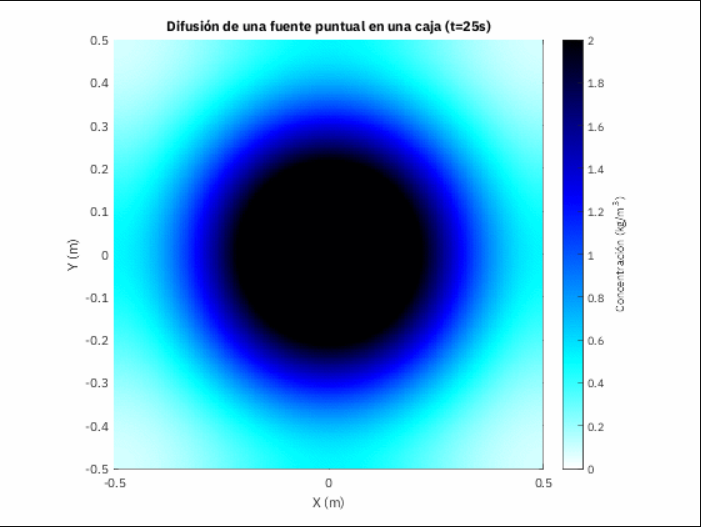
\includegraphics[width=.3\paperwidth]{E_IMAGENES/1_Capitulo2/25.png}\qquad
    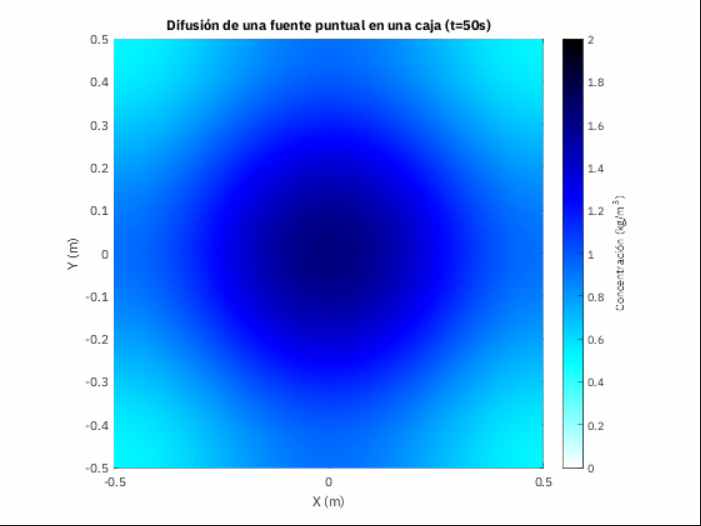
\includegraphics[width=.3\paperwidth]{E_IMAGENES/1_Capitulo2/50.png}
    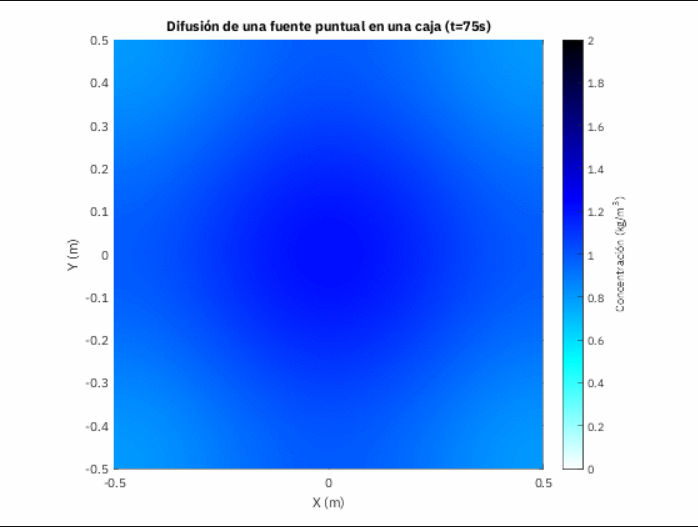
\includegraphics[width=.3\paperwidth]{E_IMAGENES/1_Capitulo2/75.png}\qquad
    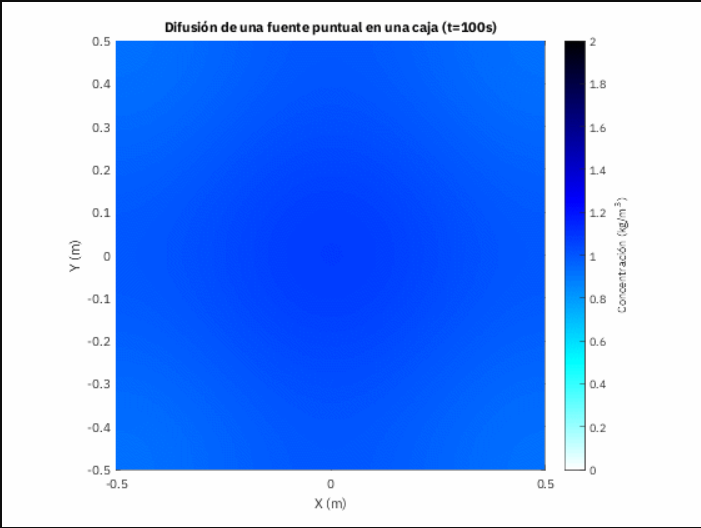
\includegraphics[width=.3\paperwidth]{E_IMAGENES/1_Capitulo2/100.png}
    \caption[corto]{Un tinte que se difunde en el agua en los tiempos
        $25$s, $50$s, $75$s y $100$s.
        En promedio, las partículas se mueven de regiones de mayor a menor densidad.}
\end{figure}

\begin{table}[ht!]
    \centering
    \begin{tabular}{ll}
        \textbf{Convección}                              &
        \textbf{Difusión}                                  \\
        Transporte de la magnitud por el flujo           &
        Efecto de las colisiones moleculares               \\
        \hline
        No existe en un fluido en reposo                 &
        Existe en un fluido en reposo                      \\
        \hline
        Comportamiento direccional                       &
        Comportamiento isotrópico                          \\
        \hline
        Derivadas espaciales de primer orden             &
        Derivadas espaciales de segundo orden              \\
        \hline
        No lineal, la velocidad del flujo depende de $U$ &
        Lineal, propiedades del fluido constantes
    \end{tabular}
    \caption[short]{Diferencias entre la convección y difusión.}
\end{table}

\begin{definition}[Concentración media]
    Sea $h>0$, $h\ll 1$.
    Definimos la \emph{concentración media}
    \begin{math}
        \averageconcentration
    \end{math}
    in a space-time cell
    \begin{math}
        \left[
            x-\frac{1}{2}h,
            +x\frac{1}{2}h
            \right]
        \times
        \left[
            0,T
            \right]
    \end{math}.

    \begin{equation*}
        \averageconcentration=
        \dfrac{1}{h}
        \int_{x-\frac{1}{2}h}^{x+\frac{1}{2}h}
        u
        \left(
        s,t
        \right)
        \dl s.
    \end{equation*}
\end{definition}

Sea
\begin{math}
    u\left(x,t\right)
\end{math}
la función concentración o densidad de alguna sustancia química.

\begin{definition}[Ecuación lineal de Advección-Difusión-Reacción]
    Para cualquier $x\in\Omega$ y $t\in\left[0,T\right]$,
    \begin{equation}\label{eq:advecion-difussion-reaction}
        \diffp{\phi}{t}\left(x,t\right)+
        u\left(x\right)\cdot
        \nabla\phi\left(x,t\right)=
        \nabla\cdot\left(a\left(x\right)\nabla\phi\left(x,t\right)\right)-
        c\left(x\right)\phi\left(x,t\right)
        +f\left(x,t\right)
    \end{equation}
\end{definition}

\begin{description}
    \item[Advección-Difusión]
        Si $u\equiv0$, entonces
        \begin{equation*}
            \diffp{\phi}{t}\left(x,t\right)=
            \nabla\cdot\left(a\left(x\right)\nabla\phi\left(x,t\right)\right)-
            c\left(x\right)\phi\left(x,t\right)
            +f\left(x,t\right)
        \end{equation*}

    \item[De difusión]
        Si $u\equiv0$, $c\equiv0$ y $f\equiv0$, entonces

        \begin{equation*}
            .
        \end{equation*}

    \item[De transporte lineal]

        \begin{equation*}
            .
        \end{equation*}
\end{description}

\begin{theorem}[Identidades integrales]
    Sea
    \begin{math}
        \Omega\subset
        \mathbb{R}^{d}
    \end{math}
    un dominio acotado con frontera suficientemente suave
    y
    \begin{math}
        n\colon
        \partial\Omega\to
        \mathbb{R}^{d}
    \end{math}
    normal unitario hacia afuera.
    Se cumplen
    \begin{description}
        \item[Integración por partes.]

            Si $u,v\in C^{1}\left(\overline{\Omega}\right)$, entonces
            \begin{equation*}
                \int_{\Omega}\diffp{u\left(x\right)}{x_{i}}
                v\left(x\right)\dl x=
                \int_{\partial\Omega}
                u\left(x\right)
                v\left(x\right)
                n\left(x\right)\cdot
                e_{i}
                \dl{S\left(x\right)}-
                \int_{\Omega}u\left(x\right)
                \diffp{v\left(x\right)}{x_{i}}
                \dl x.
            \end{equation*}

        \item[Primera identidad de Green.]
            Si $v\in C^{1}\left(\overline{\Omega}\right)$ y
            $w\in C^{2}\left(\overline{\Omega}\right)$, entonces
            \begin{equation*}
                \int_{\Omega}\nabla v\left(x\right)\cdot
                w\left(x\right)\dl x=
                -\int_{\Omega}
                v\left(x\right)
                \Delta w\left(x\right)
                \dl x+
                \int_{\partial\Omega}
                v\left(x\right)
                \diffp{w\left(x\right)}{n}
                \dl{S\left(x\right)},
            \end{equation*}
            donde
            \begin{math}
                \diffp{w\left(x\right)}{n}=
                n\left(x\right)\cdot
                \nabla w\left(x\right)
            \end{math}.

        \item[Segunda identidad de Green.]

            Si $v,w\in C^{2}\left(\overline{\Omega}\right)$, entonces
            \begin{equation*}
                \int_{\Omega}
                \left(
                v\left(x\right)
                \Delta w\left(x\right)-
                \Delta v\left(x\right)
                w\left(x\right)
                \right)
                \dl x=
                \int_{\partial\Omega}
                \left(
                v\left(x\right)
                \diffp{w}{n}\left(x\right)-
                \diffp{v}{n}\left(x\right)
                w\left(x\right)
                \right)
                \dl{S\left(x\right)}.
            \end{equation*}

        \item[]

            Si $v\in C^{1}\left(\overline{\Omega};\mathbb{R}^{d}\right)$ y
            $w\in C^{1}\left(\overline{\Omega}\right)$, entonces
            \begin{equation*}
                \int_{\Omega}\nabla\cdot v\left(x\right)
                w\left(x\right)
                \dl x=
                \int_{\partial\Omega}
                v\left(x\right)\cdot
                n\left(x\right)
                w\left(x\right)
                \dl{S\left(x\right)}-
                \int_{\Omega}
                v\left(x\right)\cdot
                \nabla w\left(x\right)
                \dl x.
            \end{equation*}
    \end{description}
\end{theorem}

La conservación de la masa conlleva a la ecuación de continuidad.

\subsection{Aproximaciones de diferencias finitas de las derivadas}

Si $u\colon\mathbb{R}^d\to\mathbb{R}$ es una función suficientemente
suave y
\begin{equation*}
    \forall i=1,\dotsc d:\quad
    \diffp{u\left(x\right)}{x_{i}}=
    \lim\limits_{h\to0}
    \dfrac{
        u\left(x+he_{i}\right)-
        u\left(x\right)}{h},
\end{equation*}

donde $e_{i}$ es el $i$-ésimo vector de la base canónica de
$\mathbb{R}^d$.

El método de las diferencias finitas surge al aproximar la derivada
de una función por una expresión de diferencias de valores de esta en
ciertos puntos discretos cercanos, y así, convertimos una ecuación
diferencial en un sistema finito de ecuaciones algebraicas que puede
ser resuelto en la computadora.
La elección de esta ``diferencia finita'' debería ser

\begin{description}
    \item[Consistente:]

        La aproximación sea tan precisa como sea posible y encontrar
        una aproximación de diferencia finita de las derivadas que
        sea consistente con el orden más alto posible.

    \item[Estable:]

        No solo con respecto a perturbaciones de los datos, sino
        en las versiones discretas de las mismas normas en las que la
        solución al problema continuo posee sus propias propiedades
        estabilidad.
\end{description}

% TODO: p. 103. [Hundsdorfer]
Una condición necesaria para la estabilidad es que el dominio de
dependencia de la ecuación diferencial parcial esté contenida en el
dominio de dependencia numérico, y en los problemas lineales es
conocido como

% TODO: p. 46 [Lax].
\begin{theorem}[Teorema de Equivalencia de Lax-Richtmyer]
    Un problema de valor inicial bien planteado y una aproximación de
    diferencia finita que satisface la condición de consistencia y
    estabilidad es una condición necesaria y suficiente para la
    convergencia.
\end{theorem}

\begin{figure}[ht!]
    \centering
    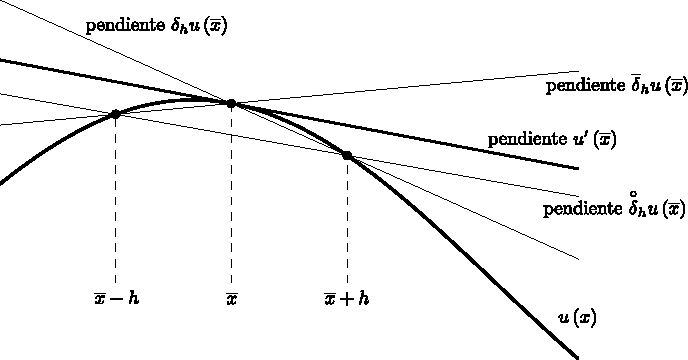
\includegraphics[width=.5\paperwidth]{E_IMAGENES/1_Capitulo2/finite_difference.pdf}
    \caption{
        Ilustración de los operadores de diferencias finitas usuales.
        Adaptado de~\citep{leveque_numerical_1992}.
    }
\end{figure}

Ahora, presentaremos algunas definiciones generales acerca de las
discretizaciones que nos permitirá estudiar la consistencia y
estabilidad de los esquemas venideros.

\subsection{Consistencia y Estabilidad de los Métodos de Diferencias Finitas}

Sean
\begin{math}
    \left(
    \mathbb{V},
    {\left\|\cdot\right\|}_{\mathbb{V}}
    \right)
\end{math},
\begin{math}
    \left(
    \mathbb{F},
    {\left\|\cdot\right\|}_{\mathbb{F}}
    \right)
\end{math}
y
\begin{math}
    \left(
    \mathbb{G},
    {\left\|\cdot\right\|}_{\mathbb{G}}
    \right)
\end{math}
tres espacios normados, donde el primero es de funciones definidas
sobre $\overline{\Omega}={\left[0,1\right]}^{d}$.
Encuentre un $u\in\mathbb{V}$ tal que
\begin{equation}\label{eq:boundary_value_problem}
    \begin{cases}
        Lu=f,     & \text{ en }\Omega,         \\
        \ell u=g, & \text{ en }\partial\Omega,
    \end{cases}
\end{equation}
donde $L$ y $\ell$ son operadores diferenciables.
El primero está asociado con la ecuación diferencial y el segundo con
las condiciones de frontera.
Las funciones $f\colon\Omega\to\mathbb{R}$ y
$g\colon\partial\Omega\to\mathbb{R}$
son elementos de $\mathbb{F}$ y $\mathbb{G}$, respectivamente.

Encuentre un $w\in\mathcal{V}\left(\overline{\Omega}_{h}\right)$ tal
que
\begin{equation}\label{eq:boundary_value_problem_finite}
    \begin{cases}
        L_{h}w=f_{h},    & \text{ en }\Omega^{I}_{h}, \\
        \ell_{h}w=g_{h}, & \text{ en }\Omega^{B}_{h},
    \end{cases}
\end{equation}
donde $L_{h}$ y $\ell_{h}$ son operadores de diferencias finitas,
\begin{math}
    \Omega^{I}_{h}
\end{math}
y
\begin{math}
    \Omega^{B}_{h}
\end{math}
son los puntos malla interiores y frontera, respectivamente.

Sea
\begin{math}
    \left\{
    \left(
    \mathcal{V}\left(\overline{\Omega}_{h}\right),
    \left\|\cdot\right\|_{h}
    \right)
    \right\}_{h>0}
\end{math}
la aproximación con respecto a
\begin{math}
    \left(
    \mathbb{V},
    {\left\|\cdot\right\|}_{\mathbb{V}}
    \right)
\end{math}.

\begin{definition}[Estabilidad]
    Decimos que el MDF~\eqref{eq:boundary_value_problem_finite} es
    estable sii existen $h_{0}>0$ y $C>0$ tales que
    \begin{math}
        \forall h\in\left(0,h_{0}\right]
    \end{math},
    el problema~\eqref{eq:boundary_value_problem}
    tiene una única solución para cualquier
    \begin{math}
        \left(
        f_{h},g_{h}
        \right)\in
        \mathcal{V}\left(
        \Omega^{I}_{h}
        \right)\times
        \left(
        \mathcal{V}\left(
            \Omega^{B}_{h}
            \right)
        \right)
    \end{math}
    y
    \begin{equation*}
        \left\|w\right\|_{h}\leq
        C\left(
        \left\|f_{h}\right\|_{\mathcal{V}\left(
            \Omega^{I}_{h}
            \right)}+
        \left\|g_{h}\right\|_{\mathcal{V}\left(
            \Omega^{B}_{h}
            \right)}
        \right)
    \end{equation*}
    donde
    \begin{math}
        {\left\|\cdot\right\|}_{\mathcal{V}\left(
            \Omega^{I}_{h}
            \right)}
    \end{math}
    y
    \begin{math}
        {\left\|\cdot\right\|}_{\mathcal{V}\left(
            \Omega^{B}_{h}
            \right)}
    \end{math}
    son normas que tienen la propiedad de aproximación con respecto a
    \begin{math}
        \left(
        \mathbb{F},
        {\left\|\cdot\right\|}_{\mathbb{F}}
        \right)
    \end{math}
    y
    \begin{math}
        \left(
        \mathbb{G},
        {\left\|\cdot\right\|}_{\mathbb{G}}
        \right)
    \end{math},
    respectivamente.
\end{definition}

Sea
\begin{math}
    \left\{
    \left(
    \mathcal{V}\left(\overline{\Omega}_{h}\right),
    \left\|\cdot\right\|_{h}
    \right)
    \right\}_{h>0}
\end{math}
la aproximación con respecto a
\begin{math}
    \left(
    \mathbb{V},
    {\left\|\cdot\right\|}_{\mathbb{V}}
    \right)
\end{math}.

\begin{definition}[Operador de consistencia]
    Sea
    \begin{math}
        L\colon\mathbb{V}\to\mathbb{V}
    \end{math}
    un operador lineal, no necesariamente acotado y
    \begin{math}
        L_{h}\colon
        \mathcal{V}\left(\mathbb{Z}^{d}_{h}\right)\to
        \mathcal{V}\left(\mathbb{Z}^{d}_{h}\right)
    \end{math}
    un operador de diferencia finita.
    Definimos el error de consistencia en $v\in\mathbb{V}$
    \begin{equation*}
        \forall x\in\mathbb{Z}^{d}_{h}:
        \mathcal{E}_{h}\left[L,v\right]\left(x\right)=
        \left(L_{h}\pi_{h}v-\pi_{h}\left(Lv\right)\right)
        \left(x\right).
    \end{equation*}
    Decimos que el operador de diferencia finita $L_{h}$ es
    consistente al menos de orden $p\in\mathbb{N}$ con $L$ sii
    existen $k\in\mathbb{N}$, $h_{1}>0$ tales que para cualquier
    \begin{math}
        h\in\left(0,h_{1}\right]
    \end{math}
    y
    \begin{math}
        v\in C^{k}\left(\mathbb{R}^{d}\right)
    \end{math}
    \begin{equation*}
        {\left\|\varepsilon_{h}\left[L,v\right]\right\|}_{h}\leq
        C h^{p}.
    \end{equation*}
\end{definition}

\begin{definition}[Consistencia]
    Definimos el error de consistencia
    de~\eqref{eq:boundary_value_problem_finite}
    \begin{equation*}
        \mathcal{E}_{h}
        \left[u\right]
        \left(x\right)=
        \begin{cases}
            \left(L_{h}\pi_{h}u-f_{h}\right)\left(x\right) \\
            \left(\ell_{h}\pi_{h}u-g_{h}\right)\left(x\right)
        \end{cases}
    \end{equation*}
    donde $u\in\mathbb{V}$
    resuelve~\eqref{eq:boundary_value_problem}.
    Decimos que el MDF~\eqref{eq:boundary_value_problem_finite} es
    consistente al menos de orden $p\in\mathbb{N}$
    con~\eqref{eq:boundary_value_problem} sii existen
    $k\in\mathbb{N}$ tal que si
    \begin{math}
        u\in C^{k}\left(\overline{Omega}_{h}\right)
    \end{math},
    entonces existen $h_{1}>0$ y $C>0$ tales que
    \begin{math}
        \forall h\in\left(0,h_{1}\right]:
        {
        \left\|\mathcal{\varepsilon}_{h}\left[u\right]\right\|
        }_{\mathcal{V}\left(\Omega^{I}_{h}\right)}+
        {
        \left\|\mathcal{\varepsilon}_{h}\left[u\right]\right\|
        }_{\mathcal{V}\left(\Omega^{B}_{h}\right)}\leq
        C h^{p}
    \end{math}.
\end{definition}

\begin{proposition}[Consistencia]
    Sea $d=1$. Tenemos
    \begin{enumerate}
        \item

              El operador de diferencia hacia adelante es consistente
              sobre
              \begin{math}
                  C_{b}\left(\mathbb{R}\right)
              \end{math}
              hasta exactamente orden uno con.

        \item

              El operador de diferencia hacia atrás es consistente.

        \item

              El operador de diferencia centrada es consistente.
    \end{enumerate}
\end{proposition}

\begin{definition}[Malla uniforme]
    Sean $N\in\mathbb{N}$.
    El tamaño de la malla es
    \begin{math}
        h=
        \dfrac{1}{N+1}
    \end{math}
    y la malla uniforme es
    \begin{equation*}
        \mathbb{Z}^{d}_{h}\coloneqq
        \left\{
        hz\in\mathbb{R}^{d}\mid
        z\in\mathbb{Z}^{d}
        \right\}.
    \end{equation*}
\end{definition}

\begin{definition}[Conjunto de funciones malla]
    \begin{math}
        \emptyset\neq\mathcal{G}_{h}\subset
        \mathbb{Z}^{d}_{h}
    \end{math}
    es un dominio malla.
    Los puntos $x\in\mathcal{G}_{h}$ son los nodos o puntos de la
    malla.
    Se define el conjunto de funciones malla sobre $\mathcal{G}_{h}$
    como
    \begin{equation*}
        \mathcal{V}
        \left(\mathcal{G}_{h}\right)\coloneqq
        \left\{
        v\mid v\colon\mathcal{G}_{h}\to\mathbb{R}
        \right\}.
    \end{equation*}
    Además,
    \begin{math}
        \forall v\in\mathcal{V}\left(\mathcal{G}_{h}\right):
        \forall hi\in\mathcal{G}_{h}:
        v_{i}=
        v\left(hi\right)
    \end{math}.
\end{definition}

\begin{definition}[Espacio $\mathcal{V}_{0}\left(\overline{\Omega}_{h}\right)$]
    Sean
    \begin{math}
        \Omega=
        {\left(0,1\right)}^{d}
    \end{math},
    \begin{math}
        N\in\mathbb{N}
    \end{math},
    \begin{math}
        h=
        \dfrac{1}{\left(N+1\right)}
    \end{math}
    y
    \begin{math}
        \overline{\Omega}_{h}=
        \overline{\Omega}\cap
        \mathbb{Z}^{d}_{h}
    \end{math}.

    \begin{equation*}
        \mathcal{V}_{0}\left(\overline{\Omega}_{h}\right)\coloneqq
        \left\{
        v\in\mathcal{V}\left(\overline{\Omega}_{h}\right)
        \right\}
    \end{equation*}
\end{definition}

\begin{definition}[Operador diferencia finita]
    La aplicación
    \begin{equation*}
        \mathcal{F}_{h}\colon
        \mathcal{V}\left(\mathbb{Z}^{d}_{h}\right)\to
        \mathcal{V}\left(\mathbb{Z}^{d}_{h}\right)
    \end{equation*}
    es llamada \emph{operador de diferencia finita} sii
    \begin{equation*}
        \forall x\in\mathbb{Z}^{d}_{h}:
        \left(\mathcal{F}_{h}u\right)\left(x\right)=
        \sum_{e\in S}
        a_{e}\left(x,h\right)
        \left(\mathcal{S}_{e}v\right)
        \left(x\right),
    \end{equation*}
    donde $S\subset\mathbb{Z}^{d}_{h}$ es finito y $0\in S$.
\end{definition}

Sea un dominio espacio-temporal contenido en $\mathbb{R}^{d+1}$.

\begin{definition}[Dominio malla espacio-temporales]
    Sean
    \begin{math}
        \Omega=
        {\left(0,1\right)}^{d}
    \end{math},
    $T>0$, $K,N\in\mathbb{N}$.
    \begin{equation*}
        \overline{\mathcal{C}}^{\tau}_{h}\coloneqq
        \overline{\Omega}_{h}
        \times
        {\left[0,T\right]}_{\tau}=
        \left\{
        \left(x,t_{k}\right)\mid
        x\in\overline{\Omega}_{h},
        t_{k}=k\tau,
        k=0,\dotsc, K
        \right\}.
    \end{equation*}
\end{definition}

\begin{definition}[Interior discreto de $\overline{\mathcal{C}}^{\tau}_{h}$]
    \begin{equation*}
        \overline{\mathcal{C}}^{\tau}_{h}\coloneqq
        \Omega_{h}\times
        {\left(0,T\right)}_{\tau}.
    \end{equation*}
\end{definition}

\begin{definition}[Frontera lateral discreta]
    \begin{equation*}
        \partial_{L}
        \mathcal{C}^{\tau}_{h}\coloneqq
        \partial\Omega_{h}\times
        {\left[0,T\right]}_{\tau}.
    \end{equation*}
\end{definition}

\begin{definition}[Frontera parabólica discreta]
    \begin{equation*}
        \partial_{p}
        \mathcal{C}^{\tau}_{h}\coloneqq
        \overline{\Omega}_{h}\times
        \left\{0\right\}\cup
        \partial_{L}
        \mathcal{C}^{\tau}_{h}.
    \end{equation*}
\end{definition}

\begin{definition}[Espacio de funciones malla espacio-temporales]
    Sea $\mathcal{C}^{\tau}_{h}$ un dominio malla espacio-temporales.
    El espacio de funciones
    \begin{align*}
        \mathcal{V}
        \left(
        \overline{\mathcal{C}}^{\tau}_{h}
        \right) & =
        \left\{
        v\mid
        \overline{\mathcal{C}}^{\tau}_{h}\to\mathbb{R}
        \right\}.   \\
        \mathcal{V}
        \left(
        \mathcal{C}^{\tau}_{h}
        \right) & =
        \left\{
        v\mid
        \mathcal{C}^{\tau}_{h}\to\mathbb{R}
        \right\}.   \\
        \mathcal{V}
        \left(
        \partial_{L}\mathcal{C}^{\tau}_{h}
        \right) & =
        \left\{
        v\mid
        \partial_{L}\mathcal{C}^{\tau}_{h}\to\mathbb{R}
        \right\}.   \\
        \mathcal{V}_{0}
        \left(
        \overline{\mathcal{C}}^{\tau}_{h}
        \right) & =
        \left\{
        v\in
        \mathcal{V}\left(\overline{\mathcal{C}}^{\tau}_{h}\right)\mid
        v\left(x,t\right)=0,
        \forall\left(x,t\right)\in\partial_{L}\mathcal{C}^{\tau}_{h}
        \right\}.   \\
        \mathcal{V}
        \left(
        \overline{\Omega}_{h}
        \right) & =
        \left\{
        v^{k}\mid
        v\in
        \mathcal{V}
        \left(
        \overline{\mathcal{C}}^{\tau}_{h}
        \right),
        v^{k}\left(x\right)=
        v\left(x,k\tau\right)
        \forall x\in\overline{\Omega}_{h}
        \right\}
    \end{align*}
\end{definition}

Los espacios de funciones malla espacio-temporales pueden
identificarse como un espacio de funciones de valor función malla
espacial, o sea

\begin{align*}
    \mathcal{V}
    \left(
    \overline{\mathcal{C}}^{\tau}_{h}
    \right) & =
    \mathcal{V}
    \left(
    \left[0,T\right]_{\tau};
    \mathcal{V}
    \left(\overline{\Omega}_{h}\right)
    \right)=
    {
    \left(
    \mathcal{V}\left(\overline{\Omega}_{h}\right)
    \right)
    }^{K+1}.    \\
    \mathcal{V}_{0}
    \left(
    \overline{\mathcal{C}}^{\tau}_{h}
    \right) & =
    \mathcal{V}
    \left(
    \left[0,T\right]_{\tau};
    \mathcal{V}_{0}\left(\overline{\Omega}_{h}\right)
    \right).
\end{align*}

\begin{definition}
    Sean
    \begin{math}
        d\in\left\{1,2\right\}
    \end{math},
    \begin{math}
        p\in
        \left[1,\infty\right)
    \end{math}
    y
    \begin{math}
        q\in\left[1,\infty\right)
    \end{math}.

    \begin{align*}
        {\left\|v\right\|}_{
            L^{q}_{\tau}\left(L^{p}_{h}\right)
        }
         & =
        {\left(
        \tau\sum_{k=1}^{K}
        \left\|v^{k}\right\|^{q}_{L^{p}_{h}}
        \right)}^{\frac{1}{q}}. \\
        {\left\|v\right\|}_{L^{\infty}_{\tau}\left(L^{p}_{h}\right)}
         & =
        \max^{K}_{k=0}
        {\left\|v^{k}\right\|}_{L^{p}_{h}}.
    \end{align*}
\end{definition}

\begin{definition}[Número de Courant]
    Sea $\overline{\mathcal{C}}^{\tau}_{h}$ una malla
    espacio-temporal.
    El número de Courant parabólico es
    \begin{equation*}
        \mu=
        \dfrac{\tau}{h^{2}}.
    \end{equation*}
\end{definition}

\begin{definition}[Estabilidad condicional]
    Decimos que un método de diferencia finita es
    \emph{condicionalmente estable} sii este es estable.
\end{definition}

\begin{equation*}
    U^{n+1}_{j}=
    U^{n}_{j}-
    \dfrac{\lambda}{2}
    \left(U^{n}_{j+1}-U^{n}_{j}\right)+
    \dfrac{\lambda^{2}}{2}
    \left(
    U^{n}_{j+1}-
    2U^{n}_{j}+
    U^{n}_{j-1}
    \right)
\end{equation*}

\begin{example}[Problema de Cauchy]
    Sean $T>0$, $c\in\mathbb{R}\setminus\left\{0\right\}$,
    $f\colon\mathbb{R}\times\left(0,T\right]\to\mathbb{R}$ y
    $u_{0}\colon\mathbb{R}\to\mathbb{R}$, buscamos
    $u\colon\mathbb{R}\times\left[0,T\right]\to\mathbb{R}$
    tal que
    \begin{equation}
        \begin{cases}
            \difcp{u}{t}+
            c\difcp{u}{x}=f
             & \text{ para }
            \left(x,t\right)\in\mathbb{R}\times\left(0,T\right]. \\
            u\left(x,0\right)=u_{0}\left(x\right)
             & \text{ para }
            x\in\mathbb{R}.
        \end{cases}\label{eq:pde_transport}
    \end{equation}
\end{example}

\begin{definition}[Solución clásica]
    $u\in C\left(\mathbb{R}\times\left[0,T\right]\right)$ es la
    \emph{solución clásica} de~\eqref{eq:pde_transport} sii la
    ecuación y la condición inicial se cumplen puntualmente.
\end{definition}

\begin{theorem}[\eqref{eq:pde_transport} está bien planteado]
    Si $f\equiv0$ y $u_{0}\in C\left(\mathbb{R}\right)$, entonces
    $\exists u$ solución clásica $u$ de~\eqref{eq:pde_transport}.
    Su solución es dada por
    \begin{equation*}
        u\left(x,t\right)=
        u_{0}\left(x-ct\right).
    \end{equation*}
    Además, si $\exists p\in\left[1,\infty\right]$ tal que
    $u_{0}\in L\left(\mathbb{R}\right)$, entonces
    \begin{equation*}
        \forall t>0:
        {
        \left\|
        u\left(\cdot,t\right)
        \right\|
        }_{L^{p}\left(\mathbb{R}\right)}=
            {
                \left\|
                u_{0}
                \right\|
            }_{L^{p}\left(\mathbb{R}\right)}
    \end{equation*}
\end{theorem}

\begin{proof}
    .
\end{proof}

La solución de la ecuación de transporte homogénea

\begin{equation*}
    X^{\prime}\left(s\right)=c,\quad
    X\left(t\right)=x\quad\iff\quad
    X\left(s\right)=x+c\left(s-t\right)
\end{equation*}

La solución es

\begin{align*}
    u\left(x,t\right) & =
    u\left(X\left(t\right),t\right)      \\
                      & =
    u\left(X\left(0\right),0\right)+
    \int_{0}^{t}
    f\left(X\left(s\right),s\right)\dl s \\
                      & =
    u_{0}\left(x-ct\right)+
    \int_{0}^{t}f\left(x+c\left(s-t\right),s\right)\dl s.
\end{align*}

\begin{definition}[Esquema de Variación total decreciente (VTD)] % p. 178 leveque conservation laws
    \begin{equation*}
        \operatorname{VT}\left(\right)\leq
        \operatorname{VT}\left(\right).
    \end{equation*}
\end{definition}

\begin{theorem}
    Cualquier método TVD preserva la monotonicidad.
\end{theorem}

\begin{proof}

\end{proof}

\section*{El método de diferencias finitas para mallas estructuradas}

$\Delta x>0$ y $\Delta t>0$ tamaño de paso temporal, espacial

$x_{j}=j\Delta x$, $t_{n}=n\Delta t$

\begin{equation*}
    U^{n}_{j}\coloneqq
    u\left(j\Delta x, n\Delta t\right)
\end{equation*}

\begin{equation*}
    \difcp{u}{t}\approx
    \dfrac{U^{n+1}_{j}-U^{n}_{j}}{\Delta t}\quad
    \difcp{u}{x}\approx
    \dfrac{U^{n}_{j}-U^{n}_{j-1}}{\Delta x}
\end{equation*}

\begin{example}[Esquema de primer orden Upwind (FOU) cuando $v>0$]
    \begin{equation*}
        U^{n+1}_{j}=
        U^{n}_{j}-
        \dfrac{v\Delta t}{\Delta x}
        \left(U^{n}_{j}-U^{n}_{j-1}\right)+
        O\left(\Delta t,\Delta x\right)
    \end{equation*}
\end{example}

\begin{example}[Esquema de primer orden Upwind (FOU) cuando $v<0$]
    \begin{equation*}
        U^{n+1}_{j}=
        U^{n}_{j}-
        \dfrac{v\Delta t}{\Delta x}
        \left(U^{n}_{j+1}-U^{n}_{j}\right)+
        O\left(\Delta t,\Delta x\right)
    \end{equation*}
\end{example}

% \begin{figure}[ht!]
%     \centering
%     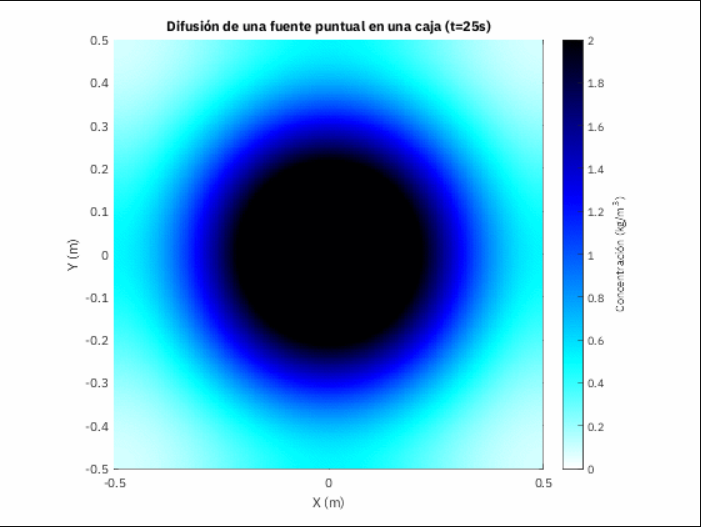
\includegraphics[width=.3\paperwidth]{E_IMAGENES/1_Capitulo2/25.png}\qquad
%     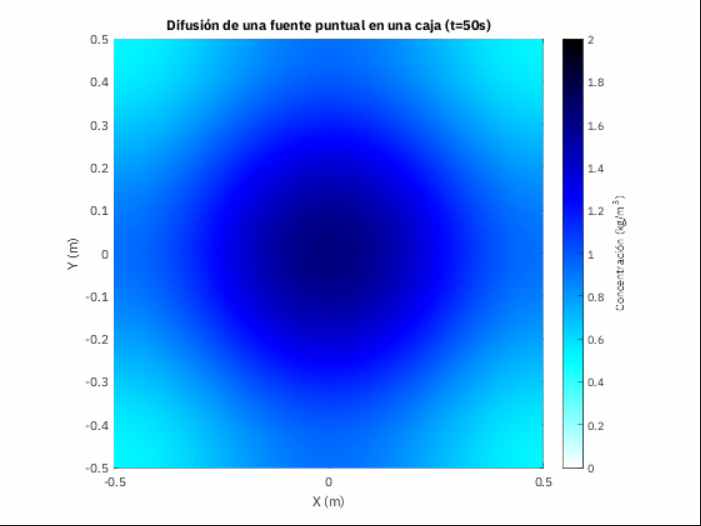
\includegraphics[width=.3\paperwidth]{E_IMAGENES/1_Capitulo2/50.png}
%     \caption[corto]{Stencil.}
% \end{figure}

$x\in\left[0,1\right]$, $U\left(x,0\right)=\exp\left(-200{\left(x-0.25\right)}^{2}\right)$

$U\left(x,t\right)=\exp\left(-200{\left(x-ct-0.25\right)}^{2}\right)$

\begin{example}[Esquema hacia adelante en tiempo, centrado en espacio (FTCS)]
    \begin{equation*}
        U^{n+1}_{j}=
        U^{n}_{j}-
        \dfrac{v\Delta t}{2\Delta x}
        \left(U^{n}_{j+1}-U^{n}_{j-1}\right)+
        O\left(\Delta t,{\left(\Delta x\right)}^{2}\right)
    \end{equation*}
\end{example}

El esquema FOU es
\begin{math}
    U^{n+1}_{j}=
    U^{n}_{j}-
    \dfrac{v\Delta t}{\Delta x}
    \left(U^{n}_{j}-U^{n}_{j-1}\right)+
    O\left(\Delta t,\Delta x\right),
\end{math}
así que reemplazamos $U^{n}_{j}$ con $U$ y $U^{n+1}_{j}$, $U^{n}_{j-1}$ con $U\left(x, t+\Delta t\right)$ y $U\left(x-\Delta x, t\right)$:
\begin{align*}
    U^{n}_{j}   & =
    U                                         \\
    U^{n}_{j-1} & =
    U-
    \Delta x\difcp{u}{x}+
    \dfrac{{\left(\Delta x\right)}^{2}}{2}
    \difcp[2]{u}{x}+
    O\left({\left(\Delta x\right)}^{3}\right) \\
    U^{n+1}_{j} & =
    U+
    \Delta t\difcp{u}{t}+
    \dfrac{{\left(\Delta t\right)}^{2}}{2}
    \difcp[2]{u}{t}+
    O\left({\left(\Delta t\right)}^{3}\right)
\end{align*}
Por lo tanto,
\begin{equation*}
    U+
    \Delta t\difcp{u}{t}+
    \dfrac{{\left(\Delta t\right)}^{2}}{2}
    \difcp[2]{u}{t}+
    O\left({\left(\Delta t\right)}^{3}\right)=
    U-
    \dfrac{v\Delta t}{\Delta x}
    \left[
        U-
        U+
        \Delta x \difcp{u}{x}-
        \dfrac{{\left(\Delta x\right)}^{2}}{2}\difcp[2]{u}{x}+
        O\left({\left(\Delta t\right)}^{3}\right)
        \right].
\end{equation*}

El esquema FTCS es
\begin{math}
    U^{n+1}_{j}=
    U^{n}_{j}-
    \dfrac{C}{2}
    \left(U^{n}_{j+1}-U^{n}_{j-1}\right),
\end{math}

donde $C=\dfrac{v\Delta t}{\Delta x}$ es el número de Courant.

El error en la aproximación numérica es $\varepsilon^{n}_{j}=U^{n}_{j}-u^{n}_{j}$ de la aproximación

\begin{equation*}
    \varepsilon^{n+1}_{j}=
    \varepsilon^{n}_{j}-
    \dfrac{C}{2}
    \left(\varepsilon^{n}_{j+1}-\varepsilon^{n}_{j-1}\right)
\end{equation*}

Esquema de Warming-Beam

\section*{Análisis de estabilidad de von Neumann}

